\documentclass[9pt, english]{beamer}
\mode<presentation>{
%\usecolortheme[overlystylish]{albatross}
\usetheme{Warsaw}
\setbeamercovered{transparent} \setbeamertemplate{navigation
symbols}{} \setbeamertemplate{footline}
{%
\leavevmode%
\hbox{%
\begin{beamercolorbox}[wd=.5\paperwidth,ht=2.5ex,dp=1.125ex,right]{author
in head/foot}%
\usebeamerfont{title in head/foot}\insertshortauthor\hspace{.3cm}
\end{beamercolorbox}%
\begin{beamercolorbox}[wd=.42\paperwidth,ht=2.5ex,dp=1.125ex,left]{title
in head/foot}%
\usebeamerfont{author in head/foot}\hspace{.3cm}\insertshorttitle
\end{beamercolorbox}%
\begin{beamercolorbox}[wd=.08\paperwidth,ht=2.5ex,dp=1.125ex,center]{author in head/foot}%
\usebeamerfont{title in head/foot}\insertframenumber/\inserttotalframenumber
\end{beamercolorbox}%
}%
\vskip0pt%
} }
\AtBeginSection[]{
\begin{frame}{\insertsection}
\tableofcontents[currentsection]
\end{frame}
}
%Per il logo Qui: \logo{\includegraphics{logo_univ_salento.EPS}}
%Dove serve: \insertlogo
\usepackage{babel}
\usepackage{hyperref}
%\usepackage{latexsym}
%\usepackage{a4wide}
%\usepackage{amscd}
\usepackage{color}
\usepackage{amsmath}%center-tags centered tags at split
\usepackage{amsthm}
\usepackage{amsfonts}
\usepackage{amsxtra}
%\usepackage{pzorin}
\usepackage{graphicx}
%\usepackage{amsmath}
\usepackage{amssymb}
%\usepackage[svgnames]{xcolor}
%\usepackage{psfrag}
\usepackage[latin1]{inputenc}
\usepackage{times}
%\usepackage[usenames]{color}
\usepackage[T1]{fontenc}
% Theorem-style
%\theoremstyle{plain}
%\newtheorem{thm}{Theorem}
%\newtheorem{prop}[thm]{Proposition}
%\theoremstyle{remark}
%\newtheorem*{remark}{Remark}

\newtheorem{thm}{Theorem}
\newtheorem{prop}[thm]{Proposition}
\newtheorem{lem}[thm]{Lemma}
\newtheorem{cor}[thm]{Corollary}

\theoremstyle{definition}
\newtheorem{defi}[thm]{Definition}
\newtheorem{oss}[thm]{Remark}
\newtheorem{es}[thm]{Example}
\newtheorem{notation}[thm]{Notation}
%\newtheorem{rem}[teo]{Remark}
\newcommand{\co}{\colon\thinspace}

\newcommand{\calT}{{\cal T}}
%\newcommand{\pdue}{$\mathbb{P}^2$}
\newcommand{\RP}{\mathbb{RP}}
%\newcommand{\matN}{\mathbb{N}}
%\newcommand{\matR}{\mathbb{R}}
%\newcommand{\matK}{\mathbb{K}}
%\newcommand{\matQ}{\mathbb{Q}}
\newcommand{\matA}{\mathbb{A}}
\newcommand{\matC}{\mathbb{C}}
\newcommand{\matZ}{\mathbb{Z}}
\newcommand{\meantmp}[2]{#1\langle{#2}#1\rangle}
\newcommand{\mean}[1]{\meantmp{}{#1}}
\newcommand{\bigmean}[1]{\meantmp{\big}{#1}}
\newcommand{\Bigmean}[1]{\meantmp{\Big}{#1}}
\newcommand{\biggmean}[1]{\meantmp{\bigg}{#1}}
\newcommand{\Biggmean}[1]{\meantmp{\Bigg}{#1}}


%\numberwithin{equation}{section}

% %own parameters
% \newlength{\boxparameter}
% \setlength{\boxparameter}{\textwidth}
% \addtolength{\boxparameter}{-6pt}

\definecolor{lightgrey}{rgb}{.7,.7,.7}
\newcommand{\red}[1]{\textcolor{red}{#1}}
\newcommand{\blue}[1]{\textcolor{blue}{#1}}
\newcommand{\hellgrau}[1]{\textcolor{lightgrey}{#1}}

%%%==========================================================================
\usepackage{bm}
\newcommand{\simbolovettore}[1]{{\boldsymbol{#1}}}
\newcommand{\va}{\simbolovettore{a}}
\newcommand{\vb}{\simbolovettore{b}}
\newcommand{\vc}{\simbolovettore{c}}
\newcommand{\vd}{\simbolovettore{d}}
\newcommand{\ve}{\simbolovettore{e}}
\newcommand{\vf}{\simbolovettore{f}}
\newcommand{\vg}{\simbolovettore{g}}
\newcommand{\vh}{\simbolovettore{h}}
\newcommand{\vi}{\simbolovettore{i}}
\newcommand{\vj}{\simbolovettore{j}}
\newcommand{\vk}{\simbolovettore{k}}
\newcommand{\vl}{\simbolovettore{l}}
\newcommand{\vm}{\simbolovettore{m}}
\newcommand{\vn}{\simbolovettore{n}}
\newcommand{\vo}{\simbolovettore{o}}
\newcommand{\vp}{\simbolovettore{p}}
\newcommand{\vq}{\simbolovettore{q}}
\newcommand{\vr}{\simbolovettore{r}}
\newcommand{\vs}{\simbolovettore{s}}
\newcommand{\vt}{\simbolovettore{t}}
\newcommand{\vu}{\simbolovettore{u}}
\newcommand{\vv}{\simbolovettore{v}}
\newcommand{\vw}{\simbolovettore{w}}
\newcommand{\vx}{\simbolovettore{x}}
\newcommand{\vy}{\simbolovettore{y}}
\newcommand{\vz}{\simbolovettore{z}}
%% \newcommand{\zero}{\simbolovettore{o0}}
\newcommand{\zero}{\boldsymbol{0}}







\newcommand{\N}{\mathbb{N}}                     % the natural numbers
\newcommand{\Z}{\mathbb{Z}}                     % the integer numbers
\newcommand{\Q}{\mathbb{Q}}                     % the rational numbers
\newcommand{\R}{\mathbb{R}}                     % the real line
\newcommand{\C}{\mathbb{C}}                     % the complex plane
\newcommand{\U}{\mathbb{U}}                     % the unit circle
\newcommand{\T}{\mathbb{T}}                     % the torus
\newcommand{\F}{\mathbb{F}}                     % a field
%\newcommand{\set}[2]{\left\{{#1}\mid{#2}\right\}}       % the set
\newcommand{\then}{\Rightarrow}                 % implication arrow
\newcommand{\sse}{\Leftrightarrow}              % iff arrow
\newcommand{\midi}{\frac{1}{2}}                 % one over two
%\newcommand{\proof}{{\sl Proof.}\hspace{5pt}}   % beginning of proof
\newcommand{\finedim}{\hfill $\Box$}            % end of proof
%\newcommand{\qed}{\hfill $\Box$ \bigskip}       % end of proof
\newcommand{\im}{\mathrm{Im\,}}                 % immaginary part
\newcommand{\re}{\mathrm{Re\,}}                 % real part
%\newcommand{\divergence}{\mathrm{div\,}}        % divergence
\newcommand{\dist}{\mathrm{dist\,}}             % distance
\newcommand{\Ker}{\mathrm{Ker\,}}               % Kernel
\newcommand{\coker}{\mathrm{coker\,}}           % Cokernel
\newcommand{\corank}{\mathrm{corank}\,}         % corank
\newcommand{\Span}{\mathrm{span\,}}             % span
%\newcommand{\sgn}{\mathrm{sgn\,}}               % signum
\newcommand{\diam}{\mathrm{diam\,}}             % diameter
\newcommand{\ind}{\mathrm{ind\,}}               % Fredholm index
\newcommand{\codim}{\mathrm{codim}}           % codimension
\newcommand{\var}{\mathrm{var\,}}               % total variation
\newcommand{\diag}{\mathrm{diag\,}}             % diagonal matrix
\newcommand{\essrange}{\mathrm{ess{\textstyle -}range}}      % essential range
\newcommand{\supp}{\mathrm{supp\,}}             % support
\newcommand{\conv}{\mathrm{conv\,}}             % convex hull
\newcommand{\spec}{\mathrm{spec\,}}             % spectrum
\newcommand{\graf}{\mathrm{graph\,}}            % graph
\newcommand{\lip}{\mathrm{lip\,}}       % Lipschitz norm
\newcommand{\rank}{\mathrm{rank\,}}     % rank
\newcommand{\ran}{\mathrm{ran\,}}       % range
\newcommand{\cat}{\mathrm{cat}}         % category
\newcommand{\Diff}{\mathrm{Diff}}       % diffeomorphisms group
\newcommand{\Sym}{\mathrm{Sym}}         % symmetric matrices
\newcommand{\dom}{\mathrm{dom}\,}       % domain
\newcommand{\esc}{\mathrm{esc}}         % essential commutator
\newcommand{\ang}{\mathrm{ang\,}}       % angle
\newcommand{\CP}{\mathbb{CP}}           % complex projective space
%\newcommand{\RP}{\mathbb{RP}}           % real projective space
\newcommand{\ps}{{\bf PS}}          % Palais-Smale condition
\newcommand{\crit}{\mathrm{crit}}       % Critical set
\newcommand{\Hom}{\mathrm{Hom}}         % Space of homomorphisms
\newcommand{\grad}{\mathrm{grad\,}}     % gradient
\newcommand{\coind}{\mathrm{coind\,}}       % co-index
\newcommand{\hess}{\mathrm{Hess\,}}     % Hessian
\newcommand{\sign}{\mathrm{sign\,}}     % signature
%\newcommand{\co}{\mathrm{co}\,}         % convex hull
\newcommand{\cco}{\mathrm{\overline{co}}\,} % closed convex hull
\newcommand{\Det}{\mathrm{Det}}                 % Determinant bundle
\newcommand{\rest}{\mathrm{rest}\,}             % set of rest poinst
\newcommand{\scal}[1]{\langle{#1}\rangle}     % scalar product
%\newcommand{\dist}{\mathrm{dist}}

\newcommand{\sixjsym}[2]{
\small{
\left|
\begin{array}{@{}c@{\ \,}c@{\ \,}c@{}}
#1 \\
#2
\end{array}
\right|
}
}
\newcommand{\twelvejsymtiny}[4]{
\tiny{
\left|
\begin{array}{@{}c@{\ \,}c@{\ \,}c@{}}
#1 \\
#2 \\
#3 \\
#4
\end{array}
\right|
}
}

\title[Stationary solutions for Kawahara diffusion equation]
{ISEM project 12}

\subtitle {Stationary solutions and their oscillating
properties for the Kawahara diffusion equation} % (optional)

\author[Virtual coordinator: Alessandro Portaluri]
{\scriptsize{\textsl{Virtual Coordinator: Alessandro Portaluri\\
Dipartimento di Matematica ``Ennio De Giorgi'', Universit\`a del
Salento, P.O.B.193, 73100, Lecce, Italy.}}\\
{\alert{alessandro.portaluri@unisalento.it}}}
%alessandro.portaluri@unisalento.it}
\institute{Team
\begin{itemize}
\item {\structure{Daniel Lengeler (Freiburg)} \texttt{daniel.lengeler@mathematik.uni-freiburg.de}}
\item {\structure{Pavel Zorin-Kranich (Pisa/T\"ubingen)} \texttt{pavel.zorin@online.de}}
\item{\structure{Wei He (Columbia)} \texttt{whgp7@mail.mizzou.edu}}
\end{itemize}
{\centerline{13th Internet Seminar on Gradient Systems, Kacov, 13-19
June 2010}}}
\begin{document}
\begin{frame}
  \titlepage
\end{frame}

\begin{frame}{Outline of the talk}
\tableofcontents
  % You might wish to add the option [pausesections]
\end{frame}

%%%%%%%%%%%%%%%%%%%%%%%%%%%%%%%%%%%%%%%%%%%%%%%%%%%%%%%%%%%%%%%%%%%%%%%%%%%%%%%%%%%%%%%%%%%%%%%%%%%%%%%%%
\section{Introduction}
\begin{frame}{Linear and nonlinear waves}
    \begin{block}{}
        Two phenomena can destroy wave packets in a \alert{homogeneous medium}:\pause
        \begin{itemize}
        \item {\structure{Dissipation}}: Fourier components are damped.\pause
        \item {\structure{Dispersion}}: Fourier components of the wave do not travel at
        the same speed.
        \end{itemize}
    \end{block}\pause
    \begin{block}{Linear theory leads to the conclusion that}\pause
        localized solutions traveling at a constant speed or solitary waves\\
        \alert{cannot exist} in a \alert{dissipative or dispersive medium.}
    \end{block}
\end{frame}
\begin{frame}{Linear and nonlinear waves}
    \begin{block}{Nonlinear theory}\pause
        ..solitary waves \alert{occur} in several areas such as
        \begin{itemize}
        \item an-harmonic nonlinear lattices,\pause
          \item gas dynamic,\pause
            \item hydromagnetic waves,\pause
              \item ion-acoustic waves in cold plasma,
                \item hydrodynamics.
        \end{itemize}
        \pause
        \alert{In all these case the nonlinearity counteracts dispersion.}
    \end{block}
\end{frame}

\begin{frame}{Aim of the project is to}
 investigate \pause
\structure{existence}, \pause
\structure{spectral stability} \pause and a
\structure{topological forcing theory} \pause
for the steady solutions of the Kawahara equation
\[
u_t=u_{xxxxx}-Pu_{xxx}-(u^{q+1})_x +c u_x, \qquad q \geq 1,
\]
%\[
%\dfrac{\partial u}{\partial t}=\dfrac{\partial^5 u}{\partial
%x^5}-P\dfrac{\partial^3 u}{\partial x^3}- \dfrac{\partial}{\partial
%x}(u^{q+1})+ c \dfrac{\partial u}{\partial x}, \qquad q \geq 1
%\]
where $P$ and $ c$ are real parameters.\pause
The importance of this equation is related to the study of water waves in presence of capillarity.\pause

    \begin{block}{The steady part}
        \[
        u_{xxxx}-Pu_{xx} + cu -u^{q+1}=0.
        \]
    \end{block}\pause
        It is also known as \structure{Swift-Hohenberg
        equation} \pause or \structure{extended Fisher-Kolmogorov
        equation} depending on the sign of the parameters.
\end{frame}

\subsection{Spectral stability and symplectic invariants}
\begin{frame}{About spectral stability}\pause
    \begin{block}{Solitary waves as homoclinic solutions}\pause
        Hamiltonian evolution equations in 1D have the property that
        their steady part is a {\color{magenta}{finite-dimensional Hamiltonian
        system.}\/}\pause Thus solitary wave solutions are homoclinic
        orbits of the associated Hamiltonian system.
    \end{block}
    \pause
    \begin{block}{Advantage of the Hamiltonian structure}\pause
        Linear and nonlinear Hamiltonian systems have {\color{magenta}{global
        geometric properties}\/} that aid in proving existence of the
        basic solitary waves \pause and in understanding its stability as a
        solution of the time dependent equation.
    \end{block}\pause
    \begin{block}{Geometric invariants}\pause
    \begin{enumerate}
    \item {\color{magenta}{Maslov index}\/}\pause
    \item {\color{magenta}{Evans function}\/}
    \end{enumerate}
    \end{block}
    \end{frame}
\subsection{Homoclinics and mountain pass}
\begin{frame}{About the existence}
    \begin{block}{Homoclinic solutions}
        for the Swift-Hohenberg-type systems are mainly based on  variational
        methods.\pause They are obtained by performing a
        {\color{magenta}{mountain-pass procedure}\/} for the associated action functional.
    \end{block}
    \pause
    \begin{block}{Main problems}\pause
        \begin{itemize}
        \item {\color{red}{Failure of the Palais-Smale condition}.\/}\pause
        \item {\color{red}{The functional is unbounded both from above and
        below.}\/}
        \end{itemize}
    \end{block}
\end{frame}
\subsection{Braids and Lagrangian dynamics}
\begin{frame}{About the forcing theory}
    \begin{block}{The Swift-Hohenberg Lagrangian}\pause
        is an example of {\color{red}{twist}\/}\pause and {\color{red}{dissipative
        system.}\/}\pause It is possible to construct a
        Morse-type theory on certain spaces of braid diagrams.\pause

        We define a {\color{magenta}{topological invariant}\/} of closed positive braids which
        is correlated with the existence of invariant sets of {\color{blue}{parabolic
        flows}\/} defined on discretized braid spaces.\pause

        Parabolic flows, a type of 1D lattice dynamics, evolve singular braid diagrams in
        such a way as to decrease their topological complexity.
    \end{block}
\end{frame}
\begin{frame}{Local versus global}
    \begin{block}{Globalization}\pause
        Algebraic lengths decrease monotonically.\pause \\ This topological
        invariant is derived from a Morse-Conley homotopy index.\pause \\
        One such well-established globalization appears in the work
        of Angenent on curve-shortening:
        \begin{quote}
        \alert {evolving closed curves on a surface by curve
        shortening isolates the classes of curves dynamically and
        implies a monotonicity with respect to a number of
        self-intersections.}
        \end{quote}
    \end{block}

\end{frame}
























%%%%%%%%%%%%%%%%%%%%%%%%%%%%%%%%%%%%%%%%%%%%%%%%%%%%%%%%%%%%%%%%%%%%%%%%%%%%%%%%%%%%%%%%%%%%%%%%%%%%%%%%%%%%%%%%

\section{Physical context and spectral stability}


\begin{frame}{Gerrida}
\begin{figure}\label{fig:gerrida}
        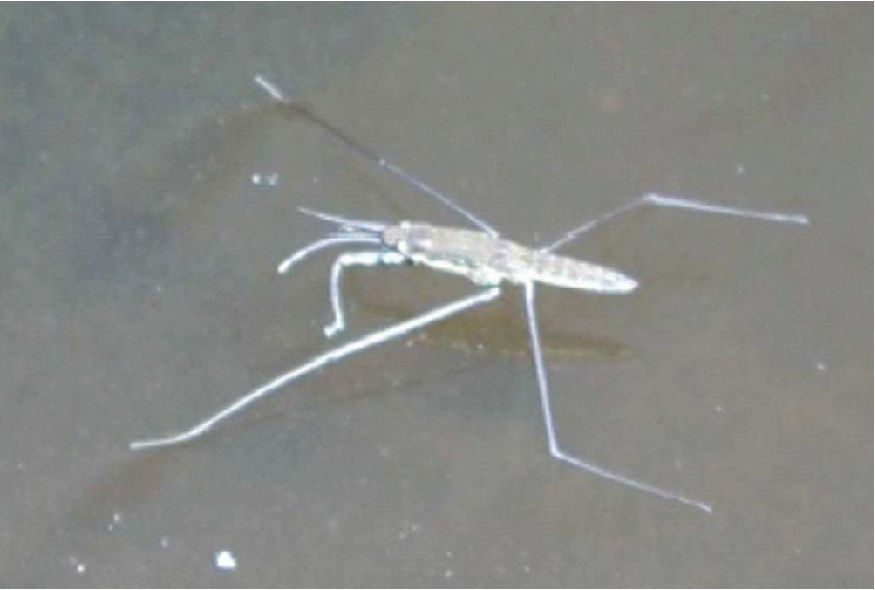
\includegraphics[width=0.9\textwidth]{images/Fig31Chardard2.pdf}
\caption{Water-strider (Gerrida) taking advantage of surface tension
        to counterbalance gravity.}
        \end{figure}
\end{frame}


\begin{frame}
  \frametitle{The Kawahara Equation}
  %\framesubtitle{Optional}
  \begin{block}{}
  $$u_t + u_x + u_{xxx} + u_{xxxxx} + (u^{q+1})_x = 0 \mbox{ for } q\ge 1$$
  \end{block}
  \begin{itemize}
   \item Higher order generalization of famous Korteweg-de Vries equation:\\ \hspace{2.5cm} $u_t + u_{xxx} + uu_x = 0$
   \item A model for (among others) propagation of low amplitude water waves in shallow canal, subject to gravity and
capillarity
   \item Hamiltonian system: solutions are orbits along the \structure{symplectic} gradient of
energy $H$, ``symplectic gradient system''\\
$\leadsto$ Conservation of energy, instead of dissipation
  \end{itemize}
\begin{block}{}
{\begin{bf} Reminder\end{bf}}: Vector space $V$, symplectic form $\omega$ on $V$, i.e.\\
\vspace{0.15cm}
\hspace{0.5cm} nondegenerate, skew-symmetric bilinear form (and $d\omega=0$),\\
\vspace{0.15cm} functional $H: V\rightarrow \mathbb{R}$. Define
$\omega(X_H,\cdot) := dH$.
$$\leadsto u_t=X_H(u)$$
\end{block}
\end{frame}

\begin{frame}
  \frametitle{Nonlinear Dispersive Equations}
  %\framesubtitle{Optional}
Linear (nondissipative) wave type equations usually exhibit  \structure{dispersion}:\\
\vspace{0.15cm}
\hspace{0.25cm} Different Fourier components of a solution travel at different speeds.\\
\vspace{0.15cm}
\begin{block}{Example}
$u(t,x)=Ae^{i(t\omega + xk)}$ solves Airy equation $u_t + u_{xxx} =
0$ iff $\omega = k^3$, i.e.$$u(t,x)=Ae^{ik(x -  (-k^2)t)}$$
\vspace{-0.5cm}
\begin{itemize}
 \item All frequencies propagate leftward
 \item Higher frequencies propagate faster than lower ones
\end{itemize}
$\leadsto$ Localised high-amplitude states disperse leftward into
broader, lower amplitude states (but conserving energy!)
\end{block}
\vspace{0.25cm} {\bf But}: Solitary waves (solitons) can be observed
in nature. $\leadsto$ Nonlinearity counteracts dispersion
\end{frame}

\begin{frame}
  \frametitle{Nonlinear Dispersive Equations}
  %\framesubtitle{Optional}
Some remarkable properties of KdV:
\begin{itemize}
 \item admits stable solitary wave solutions moving to the right, while nonlocal states move to the left
 \item colliding solitons interact nonlinearly, but emerge almost unchanged (shifted)
 \item completely integrable, roughly: infinitely many conserved quantities $\leadsto$ phase space (formally) reduces to
a point
 \item inverse scattering technique: (almost) explicit formula for solution to arbitray (sufficiently regular) initial
data
 \item generic initial data: most of the solution ``radiates'' away to the left, while finite number of solitons moving
to the right emerges
\end{itemize}
Same approach possible for gKdV, $u_t + u_{xxx} + (u^q)_x = 0$ with
$q=3$, and some NLS equations, {\bf but not} for more general
equations like gKdV with $q\not=2,3$ or the Kawahara equation.
\end{frame}

\section{Physical Derivation of the Kawahara Equation}

\begin{frame}
  \frametitle{2d-Euler equations}
  %\framesubtitle{Optional}
  Ideal, inviscid, incompressible, irrotational two-dimensional fluid with free boundary subject to capillarity and
gravity. After non-dimensionalisation:
\begin{block}{}
\begin{equation*}\begin{aligned}
  u_t + \alpha(uu_x + wu_z) + p_x &= 0,\\
 \beta [w_t + \alpha(uw_x + ww_z)] + p_z &=0,\\
 \Delta \phi &= 0,
\end{aligned}\end{equation*}
\end{block}
with velocity field $(u,w)=\nabla\phi$ in $(x,z)$ coordinates,
``pressure'' $p$, $\alpha=a/h_0$, $\beta=(h_0/l)^2$, amplitude and
wavelength $a,l$ of the surface wave, height $h_0$ of the
undisturbed surface. Boundary conditions:
\begin{block}{}
\begin{equation*}\begin{aligned}
  w&=0 \mbox{ at } z=0,\\
  w&=\eta_t+\alpha u\eta_x\mbox{ at } z=1+\alpha\eta,\\
  p&=\eta - \beta\tau\frac{\eta_{xx}}{(1+\alpha^2\beta\eta_x^2)^{3/2}}\mbox{ at } z=1+\alpha\eta,
\end{aligned}\end{equation*}
\end{block}
with free surface $h=1 + \alpha\eta$, Bond number $\tau=\Gamma/\rho
g h_0^2$, surface tension coefficient $\Gamma$, density $\rho$,
gravitional acceler. $g$.
\end{frame}

\begin{frame}
  \frametitle{Coupling of $\alpha$ and $\beta$}
  %\framesubtitle{Optional}
  {\bf Goal}: Eliminate $u,w,p$ in the small-amplitude and long-wavelength limit.\\
 \bigskip
Linearisation at $0$ and plugging $\eta=Ae^{i(\omega t - kx)}$ gives
\begin{block}{}{\small
\begin{equation*}\begin{aligned}
\omega^2 = \frac{g}{h_0}\Big((1+\tau k^2h_0^2)kh_0\tanh(kh_0)\Big)
\approx gh_0k^2\Big[1-\Big(\frac{1}{3} - \tau\Big)k^2h_0^2 +
\mbox{h.o.t.}\Big]
\end{aligned}\end{equation*}}
\end{block}
in the long wavelength limit $kh_0 \ll 1$.\\
\bigskip
$\leadsto$ Leading order dispersive term is of order
$(\frac{1}{3}-\tau)k^2h_0^2$, equiv. $(\frac{1}{3}-\tau)\beta$
\begin{block}{}
Since the nonlinearity is of order $\alpha$, we need
\begin{equation*}\begin{aligned}
  \alpha=O(\beta) &\mbox{ if } \abs{1/3-\tau}=O(1),\\
  \alpha=O(\beta^2) &\mbox{ if } \abs{1/3-\tau}=O(\beta).
\end{aligned}\end{equation*}
\end{block}
\end{frame}

\begin{frame}
  \frametitle{Eliminating $u,w,p$}
  %\framesubtitle{Optional}
  Course of action:
  \begin{itemize}
   \item Express the boundary conditions by Taylor series expansion at $z=1$:
\begin{block}{}
\vspace{-0.35cm}
\begin{equation*}\begin{aligned}
  w + \alpha\eta w_z + \frac{\alpha^2\eta^2}{2} w_{zz}&=\eta_t+\alpha\eta_x (u + \alpha\eta u_z) + O(\alpha^3) \mbox{ at
} z=1,\\
  p + \alpha\eta p_z + \frac{\alpha^2\eta^2}{2}p_{zz}&=\eta
- \beta\tau\eta_{xx} + O(\alpha^3,\alpha^2\beta^2)\mbox{ at } z=1,
\end{aligned}\end{equation*}
\end{block}
\item Expand $u,w,p,\eta$ into double power series $q=\sum_{i,j=0}^\infty \alpha^i\beta^jq_{ij}$
\item Plug expansions into Euler equations and expanded boundary conditions
\item Compare the coefficients of terms of order $O(1),O(\alpha),O(\beta),O(\alpha^2),O(\beta^2),O(\alpha\beta)$
\item Combine to get equations for $\eta_{ij}$
 \end{itemize}
\end{frame}

\begin{frame}
  \frametitle{Equations for $\eta_{ij}$}
  %\framesubtitle{Optional}
{\small\begin{equation*}\begin{aligned}
\eta_{00tt} - \eta_{00xx} &= 0\\
\eta_{10tt} - \eta_{10xx} &= \Big[\frac{\eta_{00}^2}{2} +
\Big(\int_{-\infty}^x\eta_{00t}\Big)^2\Big]_{xx}\\
\eta_{01tt} - \eta_{01xx} &= \Big(\frac{1}{3}-\tau\Big)\eta_{00xxxx}\\
\eta_{20tt} - \eta_{20xx} &= (\eta_{00}\eta_{10})_{xx} + 2
\Big[\int_{-\infty}^x\eta_{00t}\int_{-\infty}^x\eta_{10t}\Big]_{xx}
-
\Big[\eta_{00}\Big(\int_{-\infty}^x\eta_{00t}\Big)^2\Big]_{xx}\\
\eta_{02tt} - \eta_{02xx} &= \Big(\frac{1}{3}-\tau\Big)\eta_{01xxxx}
+
\frac{1}{3}\Big(\frac{2}{5}-\tau\Big)\eta_{00xxxxxx}\\
\eta_{11tt} - \eta_{11xx} &=
2\Big(\int_{-\infty}^x\eta_{00t}\int_{-\infty}^x\eta_{01t}\Big)_{xx}
+
\Big(\frac{1}{3}-\tau\Big)\eta_{10xxxx} + \frac{2}{3}(\eta_{00t}^2)_{xx} + (\eta_{00}\eta_{00xx})_{xx}\\
& \hspace{0.25cm}- \tau(\eta_{00}\eta_{00xxx})_x
\end{aligned}\end{equation*}}
\red{Combine according to $\eta=\sum_{i,j=0}^\infty
\alpha^i\beta^j\eta_{ij}$.}
\end{frame}

% \begin{frame}
%   \frametitle{Approximate equation for $\eta$}
%   %\framesubtitle{Optional}
% \begin{block}{Boussinesq type equation}
% {\begin{equation*}\begin{aligned}
% \eta_{tt}-\eta_{xx} &-\alpha\Big[\frac{\eta^2}{2} + \Big(\int_{-\infty}^x\eta_t\Big)^2 \Big]_{xx} - \beta
% \Big[\frac{1}{3} - \tau\Big]\eta_{xxxx} + \alpha^2\Big[\eta\Big(\int_{-\infty}^x\eta_t\Big)^2\Big]_{xx} \\
% &+ \alpha\beta \Big[\frac{2}{3}(\eta_t^2)_{xx} + (\eta\eta_{xx})_{xx} -\tau(\eta\eta_{xxx})_x\Big] -
% \frac{\beta^2}{3}\Big[\frac{2}{5}-\tau\Big]\eta_{xxxxxx} = 0
% \end{aligned}\end{equation*}}
% \end{block}
% \begin{itemize}
% \item Models bi-directional propagation of small-amplitude long-\\ wavelength capillarity-gravity water waves up to
% order $O(\alpha^2)$,\\ $O(\beta^2),O(\alpha\beta)$
% \item Nonlocal in space
% \item Validity not uniform in $t$ due to growth of $\eta_{ij}$
% \item Linearly well-posed for $\tau<2/5$
% \item Nonlinearity of order $O(\alpha),O(\alpha^2),O(\alpha\beta)$
% \item Dispersion of order $O(\beta),O(\beta^2)$
% \end{itemize}
% \end{frame}

\begin{frame}
  \frametitle{Approximate equation for $\eta$}
  %\framesubtitle{Optional}
\begin{block}{Boussinesq type equation}
{\begin{equation*}\begin{aligned} \eta_{tt}-\eta_{xx}
&-\alpha\Big[\frac{\eta^2}{2} + \Big(\int_{-\infty}^x\eta_t\Big)^2
\Big]_{xx} - \beta
\Big[\frac{1}{3} - \tau\Big]\eta_{xxxx} + \alpha^2\Big[\eta\Big(\int_{-\infty}^x\eta_t\Big)^2\Big]_{xx} \\
&+ \alpha\beta \Big[\frac{2}{3}(\eta_t^2)_{xx} +
(\eta\eta_{xx})_{xx} -\tau(\eta\eta_{xxx})_x\Big] -
\frac{\beta^2}{3}\Big[\frac{2}{5}-\tau\Big]\eta_{xxxxxx} = 0
\end{aligned}\end{equation*}}
\end{block}
\begin{itemize}
\item Taken into account terms of order up to $O(\alpha^2)$, $O(\beta^2),O(\alpha\beta)$
\item Validity not uniformly in $t$ due to growth of $\eta_{ij}$
\item Nonlinearity of order $O(\alpha),O(\alpha^2),O(\alpha\beta)$
\item Dispersion of order $O(\beta),O(\beta^2)$
\end{itemize}
\end{frame}

\begin{frame}
  \frametitle{Coupling of $\alpha$ and $\beta$}
  %\framesubtitle{Optional}
\begin{block}{Case 1: $\abs{1/3-\tau}\gg\beta$}
We need $\alpha=O(\beta)$. Up to order $O(\alpha)=O(\beta)$ we get
\begin{equation*}\begin{aligned}
\eta_{tt}-\eta_{xx} &-\alpha\Big[\frac{\eta^2}{2} +
\Big(\int_{-\infty}^x\eta_t\Big)^2 \Big]_{xx} \pm \alpha c_1
\eta_{xxxx} = 0
\end{aligned}\end{equation*}
\end{block}
\begin{block}{Case 2: $\abs{1/3-\tau}=O(\beta)$}
We need $\alpha=O(\beta^2)$. Up to order $O(\alpha)=O(\beta^2)$ we
get
\begin{equation*}\begin{aligned}
\eta_{tt}-\eta_{xx} &-\alpha\Big[\frac{\eta^2}{2} +
\Big(\int_{-\infty}^x\eta_t\Big)^2 \Big]_{xx} \pm \alpha c_1
\eta_{xxxx} - \alpha c_2 \eta_{xxxxxx} = 0
\end{aligned}\end{equation*}
\end{block}
\end{frame}

% \begin{frame}
%   \frametitle{Boussinesq and KdV type equations}
%   %\framesubtitle{Optional}
%   \begin{itemize}
%    \item Coord. transformation: $X=\frac{1}{\sqrt{c_1}}\Big(x+\alpha\int_{-\infty}^x\eta(y,t)dy\Big),
% T=\frac{1}{\sqrt{c_1}}t$
%    \item Substitute $N=\frac{3}{2}(\eta-\alpha\eta^2)$
%    \item Neglect terms of order $O(\alpha^2)$ and higher
%   \end{itemize}
% \begin{block}{Boussinesq type equations}
% \begin{equation*}\begin{aligned}
% \mbox{Case 1: } &N_{TT} - N_{XX} - \alpha (N^2)_{XX} \pm\alpha N_{XXXX} = 0 \\
% \mbox{Case 2: } &N_{TT} - N_{XX} - \alpha (N^2)_{XX} \pm\alpha N_{XXXX} -c_3\alpha N_{XXXXXX} = 0
% \end{aligned}\end{equation*}
% \end{block}
%   \begin{itemize}
%    \item Coord. transformation: $\xi=X-T,\tau=\alpha T$
%    \item Neglect terms of order $O(\alpha^2)$ and higher
%    \item Integrate once
%    \item Scaling of coordinates
%  \end{itemize}
% \begin{block}{KdV type equations}
% \begin{equation*}\begin{aligned}
% \mbox{Case 1: } &N_\tau + NN_\xi + N_{\xi\xi\xi} = 0 \\
% \mbox{Case 2: } &N_\tau + NN_\xi + N_{\xi\xi\xi} + N_{\xi\xi\xi\xi\xi} = 0
% \end{aligned}\end{equation*}
% \end{block}
% \end{frame}

\begin{frame}
  \frametitle{Boussinesq type equations}
  %\framesubtitle{Optional}
  \begin{itemize}
   \item Coord. transformation: $X=\frac{1}{\sqrt{c_1}}\Big(x+\alpha\int_{-\infty}^x\eta(y,t)dy\Big),
T=\frac{1}{\sqrt{c_1}}t$
   \item Substitute $N=\frac{3}{2}(\eta-\alpha\eta^2)$
   \item Neglect terms of order $O(\alpha^2)$ and higher
  \end{itemize}
\begin{block}{Boussinesq type equations}
\begin{equation*}\begin{aligned}
\mbox{Case 1: } &N_{TT} - N_{XX} - \alpha (N^2)_{XX} \pm\alpha N_{XXXX} = 0 \\
\mbox{Case 2: } &N_{TT} - N_{XX} - \alpha (N^2)_{XX} \pm\alpha
N_{XXXX} -c_3\alpha N_{XXXXXX} = 0
\end{aligned}\end{equation*}
\end{block}
Models for bi-directional propagation of small-amplitude
long-wavelength capillarity-gravity water waves
  \begin{itemize}
   \item Case 1: positive dispersive term for $1/3\ll\tau$, negative dispersive term for $0\le\tau\ll 1/3$ ($\leadsto$
ill-posed, short-wave instability)
   \item Case 2: positive dispersive term for $\tau$ slightly smaller than $1/3$, negative for $\tau$
slightly bigger than $1/3$
 \end{itemize}
\end{frame}

\begin{frame}
\frametitle{KdV type equations}
  \begin{itemize}
   \item Coord. transformation: $\xi=X-T,\tau=\alpha T$
   \item Neglect terms of order $O(\alpha^2)$ and higher
   \item Integrate once
   \item Scaling of coordinates
 \end{itemize}
\begin{block}{KdV type equations}
\begin{equation*}\begin{aligned}
\mbox{Case 1: } &N_\tau + NN_\xi + N_{\xi\xi\xi} = 0 \\
\mbox{Case 2: } &N_\tau + NN_\xi + N_{\xi\xi\xi} +
N_{\xi\xi\xi\xi\xi} = 0
\end{aligned}\end{equation*}
\end{block}
\end{frame}

























%%%%%%%%%%%%%%%%%%%%%%%%%%%%%%%%%%%%%%%%%%%%%%%%%%%%%%%%%%%%%%%%%%%%%%%%%%%%%%%%%%%%%%%%%%%%%%%%%%%%%%%%%%%%%%%%%



\section{Mountain pass geometry and an existence result }


\subsection{Variational problem}
\begin{frame}
\frametitle{The model problem}
\begin{align*}
\tilde V(v) &= \frac14 v^4 + v^3 + v^2\\
0 &= D^4 v + \beta D^2 v + V'(v)
\end{align*}
The critical points of the Lagrange functional
\[
\tilde J_\beta(v) = \int_\R |v''|^2 / 2 - \beta |v'|^2 / 2 + \tilde
V(v), \quad v \in H^2(\R),
\]
are characterized by
\[
0 = \left\langle \tilde J_\beta'(v), \phi \right\rangle = \int_\R
v'' \phi'' - \beta v' \phi' + \tilde V'(v) \phi
\]
for every $\phi \in H^2$ and are solutions of the differential
equation.
\end{frame}

\subsubsection{Regularity of the solutions}
\begin{frame}
\frametitle{The finite difference (``discrete differentiation'')
operator}
\begin{definition}
The \emph{shift} operator:
\[
\tau_h u(x) = u(x+h).
\]
The \emph{finite difference} operator:
\[
\Delta_h u(x) = \frac{u(x+h) - u(x)}{h}.
\]
\end{definition}
Elementary properties:
\begin{align*}
\Delta_h(v u) &= (\tau_h v) \Delta_h u + (\Delta_h v) u & \text{(Leibnitz rule),}\\
\int_\R v \Delta_h u &= - \int_\R (\Delta_{-h} v) u & \text{(Partial
integration)}.
\end{align*}
\end{frame}

\begin{frame}
\frametitle{Basic tool for proving differentiability}
\begin{lemma}
Let $u \in L^2_{loc}(\R)$ be such that for any bounded interval
$\Omega$
\[
\int_\Omega |\Delta_h u|^2 \leq C_\Omega \quad \text{for every }
h>0.
\]
Then $u' \in L^2_{loc}$.
\end{lemma}
\begin{proof}
As smooth test functions $\phi$ are dense in $L^2(\Omega)$, it
suffices to observe
\begin{multline*}
\left| \int_\Omega u' \phi \right| = \left| \int_\Omega u \phi'
\right| = \left| \lim_{h \to 0} \int_\Omega u (\Delta_{-h} \phi)
\right|
\\=
\lim_{h \to 0} \left| \int_\Omega (\Delta_{h} u) \phi \right| \leq
C_\Omega ||\phi||_2. \qedhere
\end{multline*}
\end{proof}
\end{frame}

\begin{frame}
\frametitle{Regularity of solutions of the variational problem}
\[
0 = \int_\R v'' \phi'' - \beta v' \phi' + \tilde V'(v) \phi
\]
Observe that $f = \tilde V'(v) \in L^2(\R)$ by the Sobolev embedding
theorem.

Substitute $\Delta_{-h} \phi$ for $\phi$ and use partial
integration:
\[
\int_\R (\Delta_h v'') \phi'' - \underbrace{\beta (\Delta_h v')
\phi'}_{\uncover<2->{\text{unimportant}}} + f (\Delta_{-h} \phi) =
0.
\]
\pause Specialize to $\phi = \eta^4 \Delta_h v$, where $\eta$ is a
smooth positive function with compact support which is $1$ on some
interval $\Omega$ such that $|\eta'| < 1$.
\end{frame}

\begin{frame}
\frametitle{Regularity of solutions of the simplified problem}
\[
\int_\R (\Delta_h v'') (\eta^4 \Delta_h v)'' + f (\Delta_{-h}
(\eta^4 \Delta_h v)) = 0.
\]
\begin{align*}
\int \eta^4 |\Delta_h v''|^2 &\lesssim
\int \eta^2 |\Delta_h v''| |\Delta_h v' + \Delta_h v|\\
&+ \int |f| (\Delta_{-h}\Delta_h v)| + \int |f| |\Delta_h v |.
\end{align*}
\pause Use the elementary inequality $2AB \leq \epsilon A^2 +
B^2/\epsilon$. For example,
\[
\int \eta^2 |\Delta_h v''| |\Delta_h v'| \leq \epsilon \int \eta^4
|\Delta_h v''|^2 + \frac1\epsilon \int |\Delta_h v|^2.
\]
\pause If $\epsilon$ is small enough, the first term is absorbed on
the left. Procedding similarly,
\[
\int \eta^4 |\Delta_h v''|^2 \lesssim \int |\Delta_h v'|^2 + \int
|\Delta_h v|^2 + \int |f|^2 + \int |\Delta_{-h}\Delta_h v|^2.
\]
\end{frame}

\begin{frame}
\frametitle{$L^2$ estimate for the finite difference operator}
\newcommand{\dif}{\text{d}}
Finite difference operator is bounded by the differentiation
operator in norm:
\begin{align*}
\int_\R |(\Delta_h u)(x)|^2 \dif x &= \int_\R \left| \frac{1}{h}
\int_{y=x}^{x+h} u'(y) \dif y
\right|^2 \dif x\\
&\leq \int_\R \left| \frac{1}{h} \left(\int_{y=x}^{x+h} |u'(y)|^2
\dif y \right)^{1/2} h^{1/2}
\right|^2 \dif x\\
&= \frac{1}{h} \int_\R \int_{y=x}^{x+h} |u'(y)|^2 \dif y
\dif x\\
&= \int_\R |u'(x)|^2 \dif x
\end{align*}
\pause
\[
\int \eta^4 |\Delta_h v''|^2 \lesssim \int |v''|^2 + \int |v'|^2 +
\int |f|^2 = \text{constant independent of } h
\]
By the regularity lemma, $v''' \in L^2$.
\end{frame}

\begin{frame}
\frametitle{Results so far} We have shown that a critical point of
\[
\tilde J_\beta(v) = \int_\R |v''|^2 / 2 - \beta |v'|^2 / 2 + \tilde
V(v), \quad v \in H^2(\R)
\]
is in fact smooth and is a classical solution of
\begin{align*}
\tilde V(v) &= \frac14 v^4 + v^3 + v^2\\
0 &= D^4 v + \beta D^2 v + V'(v).
\end{align*}
\end{frame}

\subsection{Mountain pass geometry}
\begin{frame}
\frametitle{Equilibrium point: a mountain pass}
\includegraphics[width=0.9\textwidth]<1>{images/mountain_pass_1.jpg}
\includegraphics[width=0.9\textwidth]<2>{images/mountain_pass_2.jpg}
\includegraphics[width=0.9\textwidth]<3>{images/mountain_pass_3.jpg}
\includegraphics[width=0.9\textwidth]<4>{images/mountain_pass_4.jpg}
\includegraphics[width=0.9\textwidth]<5>{images/mountain_pass_5.jpg}
\end{frame}

\begin{frame}
\frametitle{Existence of an approximate mountain pass}
\begin{theorem}
Let $H$ be a Hilbert space, $h \in C^2(H)$, $x_0,x_1 \in H$ such
that $h(x_0) = h(x_1) = 0$, but
\begin{equation}
\inf_\gamma \max_t h(\gamma(t)) = H > 0,
\end{equation}
the infimum being taken over continuous paths $\gamma$ from $x_0$ to
$x_1$.

Then there exist points $x$ with, simultaneously, $h(x)$ arbitrarily
close to $H$ and $h'(x)$ arbitrarily close to $0$.
\end{theorem}
\pause
\begin{proof}
Assume not. Then, in some region $\{ |h-H| < 2 \epsilon \}$, $|h'|$
is bounded from below by $\epsilon$. Take a path $\gamma$ such that
\[
\max_t h(\gamma(t)) < H + \epsilon.
\]
The next lemma allows to construct a path $\tilde\gamma$ with
maximal height smaller then $H$, a contradiction.
\end{proof}
\end{frame}

\begin{frame}
\frametitle{Deformation lemma}
\begin{lemma}
Let $H$ be a Hilbert space and $h \in C^1 (H)$, $h' \in
\text{Lip}_\text{loc}$ be the height function.

Assume $|h'|>\epsilon$ in $\{ |h - H| \leq 2 \epsilon \}$.

Then there exists a flow $\eta : [0,2 \epsilon] \times H \to H$
which
\begin{itemize}
\item leaves $\{ |h - a| > 2 \epsilon \}$ fixed,
\item after time $2\epsilon$, maps $\{ h < a + \epsilon\}$ into $\{ h \leq a - \epsilon \}$.
\end{itemize}
\end{lemma}
\end{frame}

\begin{frame}
\frametitle{Deformation lemma, proof}
\includegraphics[width=0.5\textwidth]<1>{images/mountain_pass_qd_0.jpg}
\includegraphics[width=0.5\textwidth]<2>{images/mountain_pass_qd_2.jpg}
\includegraphics[width=0.5\textwidth]<3>{images/mountain_pass_qd_3.jpg}

\begin{itemize}
\item<2-> Cutoff function $g(x) := \frac{\dist(x,\complement A)}{\dist(x,\complement A) + \dist(x,B)}$.
\begin{itemize}
\item $g|_{\color{magenta} B} \equiv 1$, $g|_{\color{red} \complement A} \equiv 0$ and $g$ is locally Lipschitz.
\end{itemize}

\item<3-> Locally Lipschitz vector field ${\color{blue}X}(x) = - \frac{h'(x)}{|h'(x)|^2} g(x)$.
\begin{itemize}
\item Picard-Lindel\"of Theorem $\implies$ $X$ defines a unique continuous flow $\eta$.
\item $X$ bounded $\implies$ the flow $\eta$ exists for all times.
\item ${\color{blue} X} h|_{\color{magenta} B} = -1$.
\end{itemize}

\item<3-> Thus the time $2 \epsilon$ map of the flow $\eta$ maps $B$ into $\{ h \leq a - \epsilon \}$.
\end{itemize}
\end{frame}


\begin{frame}
\frametitle{Deformation lemma, local version}
\begin{lemma}
Let $H$ be a Hilbert space and $h \in C^1 (H)$, $h' \in
\text{Lip}_\text{loc}$ be the height function. \uncover<2->{Let
{\color{red} $S \subset H$}.}

Assume $|h'|>\epsilon$ in $\{ |h - H| \leq 2 \epsilon \}$
\uncover<2->{{\color{red} $\cap \{ \dist (\cdot,S) \leq 4 \}$}}

Then there exists a flow $\eta : [0,2 \epsilon] \times H \to H$
which
\begin{itemize}
\item leaves $\{ |h - a| > 2 \epsilon \}$
\uncover<2->{{\color{red} and $\{ \dist (\cdot,S) > 4 \}$}} fixed,
\item after time $2\epsilon$, maps $\{ h < a + \epsilon\}$
\uncover<2->{{\color{red} $\cap S$}} into $\{ h \leq a - \epsilon
\}$.
\end{itemize}
\end{lemma}

\uncover<3->{
\begin{proof}
\[
\text{Use a cutoff function which satisfies}
\phi(x) =
\begin{cases}
1, & \dist(x, S) \leq 2\\
%2 - \dist(x, S)/2, & 2 < \dist(x, S) < 4\\
0, & \dist(x, S) \geq 4.
\end{cases}
\]
Proceed as before, but use the vector field $\phi X$. As the vector
field is uniformly bounded, the flow lines starting in $S$ will stay
in $\{\dist(\cdot, S) \leq 2\}$ long enough, so that $\phi X h = -1$
where needed.
\end{proof}
}
\end{frame}

\subsection{Lagrange functional with mountain pass structure}
\begin{frame}
\frametitle{A version of the Lagrange functional with mountain pass
structure} $\tilde J_\beta$ doesn't have the mountain pass
structure.

To overcome this difficulty, we will consider a cut-off potential
and the corresponding functional
\begin{align*}
V(v) &=
\begin{minipage}{6cm}
$\begin{cases}
v^4 / 4 + v^3 + v^2 & v \geq -2\\
0 & v < -2,
\end{cases}$
\end{minipage}
\\
J_\beta(v) &= \int_\R |v''|^2 / 2 - \beta |v'|^2 / 2 + V(v).
\end{align*}
A critical point $v$ of $J_\beta$ is also a critical point of
$\tilde J_\beta$ if only it satisfies the pointwise inequality
$v>-2$. In such a case it is also a classical solution of our
equation.
\end{frame}


\begin{frame}
\frametitle{Mountain pass structure of $J_\beta$: valley at $0$} We
work in a fixed range $0 < \beta_{min} < \beta < \beta_{max} < \sqrt
8$.
\begin{lemma}
For some $\epsilon > 0$, $\delta > 0$
\[
J_\beta(v) \geq \epsilon ||v||_{H^2}^2, \quad \text{whenever } ||v||
< \delta.
\]
\end{lemma}
\begin{proof}
Sobolev embedding theorem and a calculation.
\end{proof}
\end{frame}

\begin{frame}
\frametitle{Mountain pass structure of $J_\beta$: a second valley}
\begin{lemma}
There exists $e \in H^2(R)$ such that $J_\beta(e)<0$ for every
$\beta \in [\beta_{min},\beta_{max}]$.
%\textbf{Probably no proof, just say the cut-off is useful}
\end{lemma}
\begin{proof}
Let $0 \not\equiv f$ be a negative smooth function with compact
support. Its dilates $f_\lambda(x)=f(\lambda x)$ satisfy.
\[
\int (f_\lambda'')^2 \sim \lambda^3, \quad \int (f_\lambda')^2 \sim
\lambda.
\]
\[
\text{Thus, for}\  \lambda>0\ \text{small,} \quad j_\beta = \frac12
\int_\R (f_\lambda'')^2 - \beta (f_\lambda')^2 < 0.
\]
As the support of $f_\lambda$ is bounded and $V(v)$ is bounded for
$v\leq 0$,
\[
J_\beta(C f_\lambda) = j_\beta C^2 + \text{const}, \quad \text{(this
is where the cut-off comes in!)}
\]
Thus, for $C$ big enough, $e = C f_\lambda$ has the required
properties.
\end{proof}
\end{frame}

\begin{frame}
\frametitle{Pass levels} Define the pass levels by
\[
H_\beta = \inf_\gamma \sup_{t} J_\beta(\gamma(t)),
\]
where the infimum is taken over continuous paths $\gamma$ from $0$
to $e$.

%Such paths shall be called \emph{admissible.}

\pause Recall
\[
J_\beta(v) = \text{(something)} - \beta \text{(something positive)}.
\]

Thus the pass level function $H_\beta$ is monotonously decreasing
and therefore differentiable almost everywhere.
\end{frame}

\begin{frame}
\frametitle{Minimizing sequence for $J_\beta'$}
\begin{lemma}
Let $\beta \in [\beta_{min}, \beta_{max}]$ be such that the
derivative $H'_\beta$ exists. Then there exists a sequence $(v_n)
\subset H^2(R)$ which satisfies
\begin{enumerate}
\item $J_\beta(v_n) = H_\beta + o(1)$,
\item $J_\beta'(v_n) = o(1)$,
\item $\frac12 ||v_n'||_2^2 \leq -2H'_\beta + 2$.
\end{enumerate}
\end{lemma}
\pause \emph{Proof}

Define the admissible region
\[
S = \{ u\ :\ \frac12 || u' ||_2^2 \leq - H'_\beta + \frac12 \}
\]
Assume the opposite. Then there exists an $\epsilon <  H_\beta/2$
such that
\[
||J'_\beta|| > 32 \epsilon \, \text{on} \, \{ |J_\beta - H_\beta| <
2 \epsilon \} \cap \{ \dist(\cdot,S) \leq 1/2 \}.
\]
\end{frame}

\begin{frame}
\frametitle{Minimizing sequence for $J_\beta'$: flow decreasing
$J_\beta$} By the local deformation lemma there exists a flow $\eta$
such that
\begin{itemize}
\item $\{ |J_\beta - H_\beta| \geq 2 \epsilon \}$ and $\{ \dist(\cdot,S) > 1/2 \}$ are let fixed,
\begin{itemize}
\item<2-> {\color{red} $0$ and $e$ are fixed}
\end{itemize}
\item $J_\beta$ decreases along $\eta$,
\item time $2\epsilon$ map maps $\{ J_\beta \leq H_\beta + \epsilon\} \cap S$ into $\{J_\beta \leq H_\beta - \epsilon\}$.
\end{itemize}
\uncover<2->{ For a contradiction, look for a path {\color{red}
$\gamma$ from $0$ to $e$} such that
\begin{itemize}
\item $\gamma \subset S$,
\item $J_\beta(\gamma) \leq H_\beta + \epsilon$.
\end{itemize}
}
\end{frame}

\begin{frame}
\frametitle{Minimizing sequence for $J_\beta'$: using
differentiability of the pass level function} Choose
$H_{\tilde\beta} < H_\beta$ later \uncover<2->{{\color{red} using
differentiability of $H_\beta$ in $\beta$.}}

By definition of $H_{\tilde\beta}$, there is a path $\tilde\gamma$
such that, for all $t$,
\[
\uncover<3->{{\color{blue} J_\beta(\tilde\gamma(t)) \leq}}
J_{\tilde\beta} (\tilde\gamma(t)) \leq H_{\tilde\beta} + (\beta -
\tilde\beta)/8 \uncover<2->{{\color{red} \leq H_\beta' + \epsilon}}
\]
For every $t$ with $J_\beta(\tilde\gamma(t)) \geq H_\beta -
(\beta-\tilde\beta)/8$, one has
\[
\frac12 ||\tilde\gamma(t)'||_2^2 =
\frac{J_{\tilde\beta}(\tilde\gamma(t)) -
J_\beta(\tilde\gamma(t))}{\beta - \tilde\beta} \leq
\frac{H_{\tilde\beta} - H_\beta}{\beta - \tilde\beta} + \frac14
\uncover<2->{{\color{red} \leq - H'_\beta + \frac12,}}
\]
\uncover<3->{i.e. {\color{blue} $\tilde\gamma \subset S = \{ u :\,
\frac12 || u' ||_2^2 \leq - H'_\beta + \frac12 \}$}}

\uncover<4->{{\color{blue} Local deformation lemma: $\gamma =
\eta_{2 \epsilon} (\tilde\gamma)$} is a path from $0$ to $e$ and
\[
J_\beta(\gamma) \leq H_\beta - \epsilon \text{ -- contradiction to
the definition of } H_\beta. \qedhere
\]
}
\end{frame}

\begin{frame}
\frametitle{Non-triviality of the weak limit} The sequence $v_n$
cannot converge to $0$ uniformly. Wlog one can assume that it is
bounded away from $0$ in the supremum norm. Assume
\[
\limsup_n (\min_x v_n(x)) \geq -1.
\]
In such a case, using $V(v) \geq v^2/4$, one obtains that $v_n$ is
bounded in $H^2$.

Shift the $v_n$ such that the shifted versions have a maximum at
$0$:
\[
w_n := \tau_{d_n} v_n, \quad d_n \ \text{such that}\  |v_n(d_n)| =
\max_x |v_n(x)|.
\]
Thus, if $w_n \rightharpoonup w$, then $w(0) \neq 0$, as point
evaluations are weakly continuous. It follows that $w$ is a critical
point of $J_\beta$.
\end{frame}


%%%%%%%%%%%%%%%%%%%%%%%%%%%%%%%%%%%%%%%%%%%%%%%%%%%%%%%%%%%%%%%%%%%%%%%%%%%%%%%%%%%%%%%%%%%%%%%%%%%%%%%%%%











%%%%%%%%%%%%%%%%%%%%%%%%%%%%%%%%%%%%%%%%%%%%%%%%%%%%%%%%%%%%%%%%%%%%%%%%%%%%%%%%%%%%%%%%%%%%%%%%%%%%%%%%%%%%%%%%%%

\section{Braids and parabolic dynamics}



\begin{frame}{Electricity in space}
\begin{figure}\label{fig:nebula}
        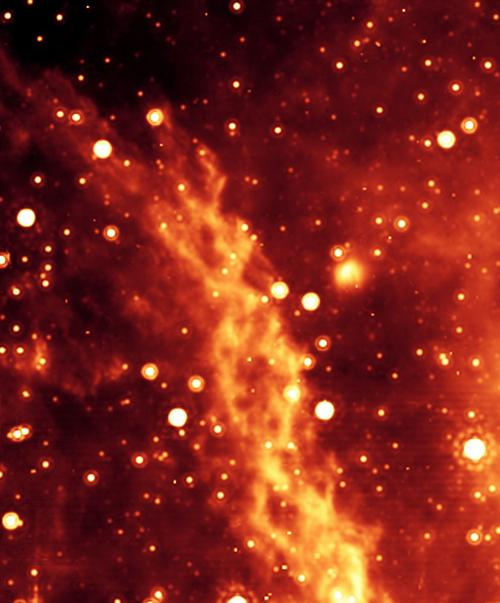
\epsfig{file=images/double-helix1-th.jpg, scale=0.3}\caption{Electric currents in space. The Double Helix nebula, located near
        our own galactic center.}
        \end{figure}
\end{frame}


\subsection{Braid-theoretic version of the comparison principle}
\begin{frame}{Perspective}
    \begin{block}{The comparison principle}
        Given a scalar uniformly parabolic PDE,
        \begin{equation}\label{eq:Wei1}
        u_t=f(x, u, u_x, u_{xx}); \ \ \textrm{where}\ \ 0<\lambda \leq
        \partial_{u_{xx}}f \leq \lambda^{-1} \textrm{uniformly}.
        \end{equation}\pause
        Assume that $f$ is of smoothness class $\mathscr C^2$ and
        for simplicity we consider only periodic boundary
        conditions. Hence $x \in S^1$.\pause \\
        We view \eqref{eq:Wei1} as an evolution equation on the
        curve $u(\cdot, t):$\pause

        \alert{as $t$ increases, the graph of $u$ evolves in the
        $(x,u)$-plane.}
    \end{block}
\end{frame}
\begin{frame}
    \begin{block}{A Comparison Principle}
        It is well-known fact (going back to Sturm, Matano, Brunovsky,
        Fiedler, Angenent, and others) that there is a \alert{comparison
        principle} for \eqref{eq:Wei1}. \pause
        In fact, if $u^1$ and $u^2$ are  solutions of \eqref{eq:Wei1},
        then the number of intersections of the graphs of $u^1$ and
        $u^2$ in the $(x,u)$-plane is a \alert{weak Lyapunov function
        for the dynamics}.
    \end{block}\pause
    \begin{block}{Total crossing numbers}
        Therefore the number
        {\color{blue}
        \[
        z_{u^1, u^2}(t)=\#\set{x}{u^1(x,t)=u^2(x,t)}
        \]\/}\pause
        is a non-increasing function of time.
    \end{block}

\end{frame}
\begin{frame}{Parabolic dynamics separates tangencies monotonically}
        %\begin{figure}
%        \centering
%        \includegraphics{file=Fig15Wojcik2.pdf, scale=0.1}\caption{The local picture of the evolution of two solutions of
%        a parabolic PDE that develop a tangency at $t_0$ [middle]. The number of intersections among the solutions
%        drops by two in a neighborhood of $t_0$.}
%        \end{figure}
        \begin{figure}\label{fig:tangencies_separation}
        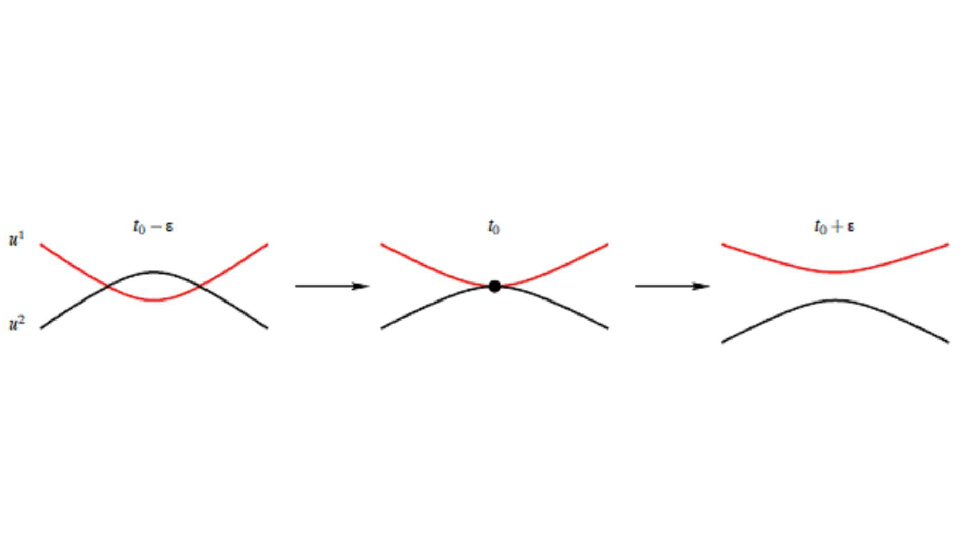
\epsfig{file=images/Fig15Wojcik2.pdf, scale=0.4}\caption{The local picture of the evolution of two solutions of
        a parabolic PDE that develop a tangency at $t_0$ [middle]. The number of intersections among the solutions
        drops by two in a neighborhood of $t_0$.}
        \end{figure}
\end{frame}
\begin{frame}{and in 1-jet extension}
    \begin{block}{one recognize the braid structure!}
        Lifting $u^1$ and $u^2$ to the $(x,u, u_x)$-space, one recognize
        a braid structure as two solutions wind around each other.
        \begin{figure}\label{fig:lift}
        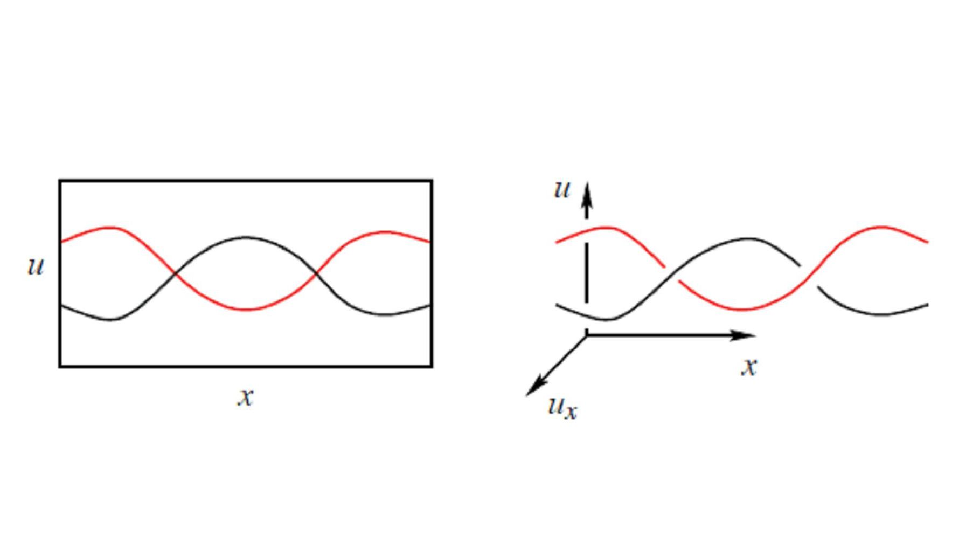
\epsfig{file=images/Fig16Wojcik21.pdf, scale=0.3}\caption{Two solutions of a parabolic equation [left]. Their lift to
        $(x,u,u_x)$-space [right].}
        \end{figure}
    \end{block}
\end{frame}
\begin{frame}{Conclusion}
    \begin{block}{Evolution of the complexity}
        Into the language of braid theory we can say that:\pause\\
        {\color{blue}
        {the evolution of the complexity of the braid corresponds to
        those solutions cannot increase.}\/}
    \end{block}
\end{frame}
\subsection{Topological and discretized braids and braids diagrams}
\begin{frame}{Braid and... }
    \begin{block}{What is a braid?}\pause
        Intuitively it is clear what a braid is! It consists of several strings that are
        intertwined.\pause
        \begin{figure}\label{fig:shoes}
        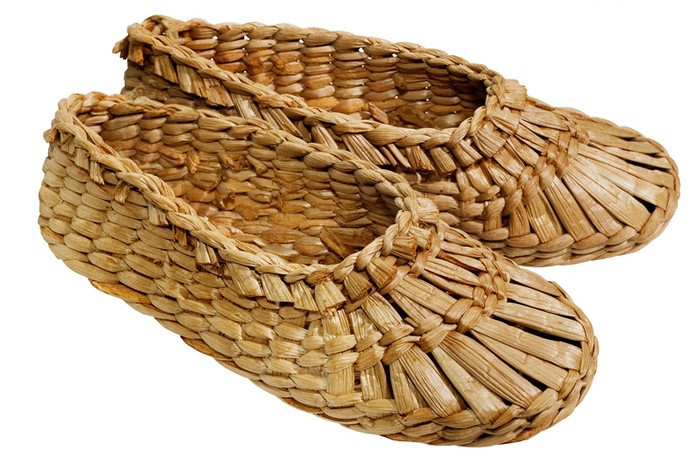
\epsfig{file=images/2774braiding_shoe.jpg, scale=0.3}\caption{Braiding shoes}
        \end{figure}
\end{block}
\end{frame}
\begin{frame}{and in mathematics?}
    \begin{block}{More precisely,}
        it is a collection of $n$ continuous curves
        $u^\alpha:[0,1] \hookrightarrow \R^3$, called
        {\color{blue}{
        strands}\/},\pause
        that are transversal to all planes parallel to one of the
        directions.\pause  For example we can assume $\partial u_1^\alpha>0$
        for all $\alpha$, where $u^\alpha=(u_1^\alpha, u_2^\alpha,
        u_3^\alpha)$.\pause Moreover, strands are assumed to have disjoint
        images {\color{red}{(they do not intersect)}.\/}
    \end{block}\pause
    \begin{block}{Closed braids}
        This does not necessarily means that all strands are
        periodic,\pause
        but that there exists a permutation $\sigma$ on $n$ elements such
        that $u^\alpha(1)=u^{\sigma(\alpha)}(0)$ for all $\alpha \in
        \{1, \dots,n\}$.
    \end{block}
\end{frame}
\begin{frame}{Notations and conventions}
        \begin{notation}
        $\vu:=\{u^1, \dots, u^n\}$.
        \end{notation}\pause
        \begin{figure}\label{fig:permutation}
        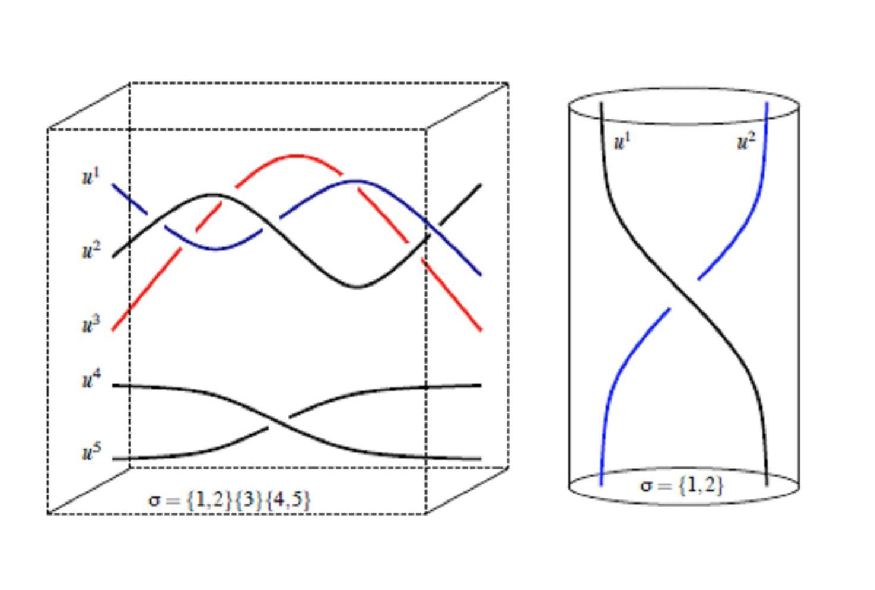
\epsfig{file=images/Fig17Wojcik21.pdf, scale=0.2}\caption{Two conventions for presenting braids.
        Horizontal- a braid on 5 strands consisting of two connected component [left]. Vertical- a braid on two strands
        (a single component)[right]. Both have the corresponding permutation indicated.}
        \end{figure}
\end{frame}
\begin{frame}{braid classes}
    \begin{oss}
        Cycles of the permutation divide braids into {\em braid
        components.\/}
    \end{oss}\pause
    \begin{block}{Equivalence relation}
        Two braids are equivalent if one can deform one into the other
        without creating any intersections along the path.\pause\\
        \color{blue}{Thus a braid class is the equivalence class of isotopic
        braids.}
    \end{block}\pause
    \begin{oss}
        Two different braid classes on $n$ strands are necessary
        separated by the so-called \alert{singular braids},\pause i.e.
        collections of curves that {\color{red}{do}\/} have intersections
        among the strands.
    \end{oss}
\end{frame}
\begin{frame}
\begin{figure}\label{fig:singular}
        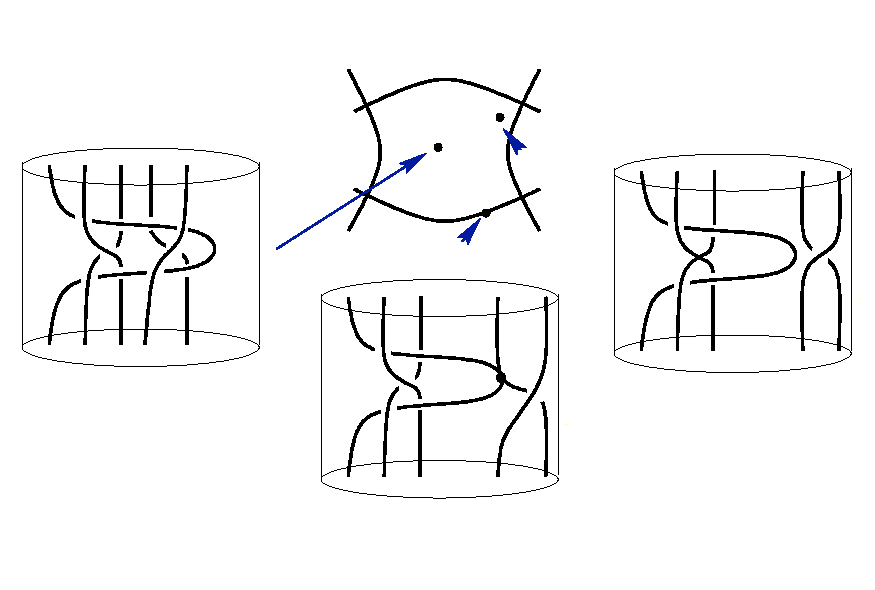
\epsfig{file=images/Fig18Wojcik.pdf, scale=0.3}\caption{Schematic picture of a braid class with two representatives indicated
        [left] and [right] and a singular one corresponding to a point on the boundary of the class [middle].}
        \end{figure}
\end{frame}
\begin{frame}{Braid diagrams }
    \begin{block}{Labeled projection}\pause
        The specification of a topological braid class \pause (closed or
        otherwise) may be accomplished unambiguously by a labeled
        projection to the $(x,u)$-plane:

        a {\color{red}{ braid diagram}\/}.\pause

        Any braid may be perturbed slightly so that pairs of strand
        crossings in the projection are transversal and disjoint.\pause
    \end{block}
        \begin{notation}
        Then mark each crossings via (+) or (-) to indicate whether the
        crossing is {\color{red}{bottom over top}\/} or {\em \color{red}{top over bottom}\/}
        respectively.\pause

        {\color{blue}{Since we are dealing with Legendrian braids all crossings have
        positive labels.}\/}
        \end{notation}
\end{frame}
\begin{frame}{Braids and their projections}
\begin{figure}\label{fig:braiddiagram}
        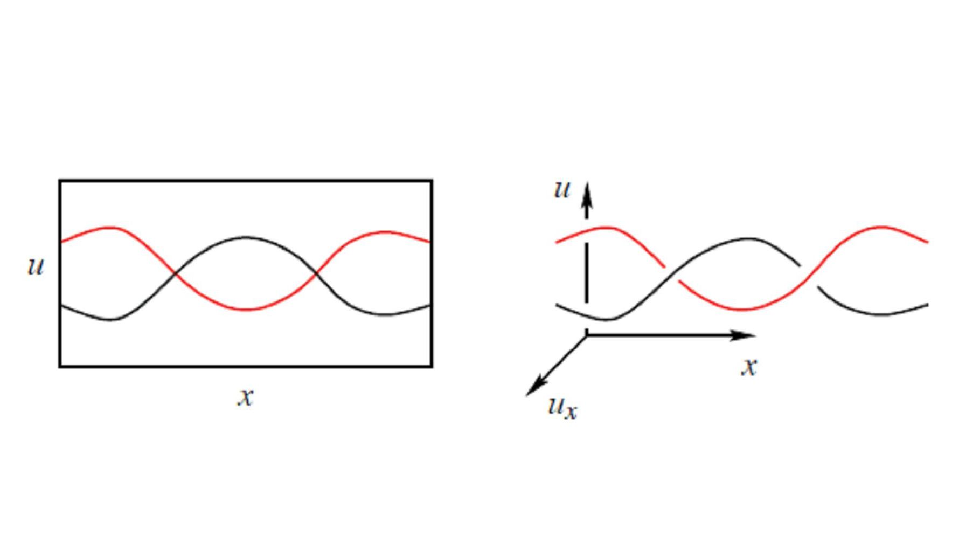
\epsfig{file=images/Fig16Wojcik21.pdf, scale=0.3}\caption{A braid on two strands [right]. The braid diagram (continuous
         representant of the class of the two dimensional projection of the braid) [right].}
        \end{figure}
\end{frame}
\begin{frame}{Topological transversality}
        \begin{block}{Definition}
            $\Omega^n$ denotes the space of all
            {\color{blue}{closed positive braid diagrams on $n$ strands pairwise
            transversal}\/}, i.e. the space of all pairs $(\vu, \tau)$ where $\tau$ is a permutation
            over $n$ elements and $\vu=\{u^\alpha(x)\}_{\alpha=1}^n$ is an unordered collection of functions of
            Sobolev class $H^1$ satisfying:
            \begin{itemize}
            \item (Periodicity): $u^\alpha(1)= u^{\tau(\alpha)}(0)$ for
            all $\alpha$;\pause
            \item (Transversality): for any $\alpha \neq \alpha'$ such
            that $u^\alpha(x_*) = u^{\alpha'}(x_*)$ for some $x_* \in
            [0,1]$, it holds that $u^\alpha(x)- u^{\alpha'}(x)$ has an
            isolated sign change at $x=x_*$.
            \end{itemize}
         \end{block}
\end{frame}
\begin{frame}
    \begin{block}{Notation}
            The braid class of a braid diagram $\vu$ is denoted by
            $\{\vu\}$.\pause

            If we allow the strands to intersect disregarding the
            second condition we obtain the closure
            $\overline \Omega^n$. Moreover the discriminant $\Sigma^n:= \overline \Omega^n \backslash \Omega^n$
            defines the {\color{red}{ singular braid diagrams}\/}.\pause
    \end{block}
        \begin{figure}\label{fig:discretized}
            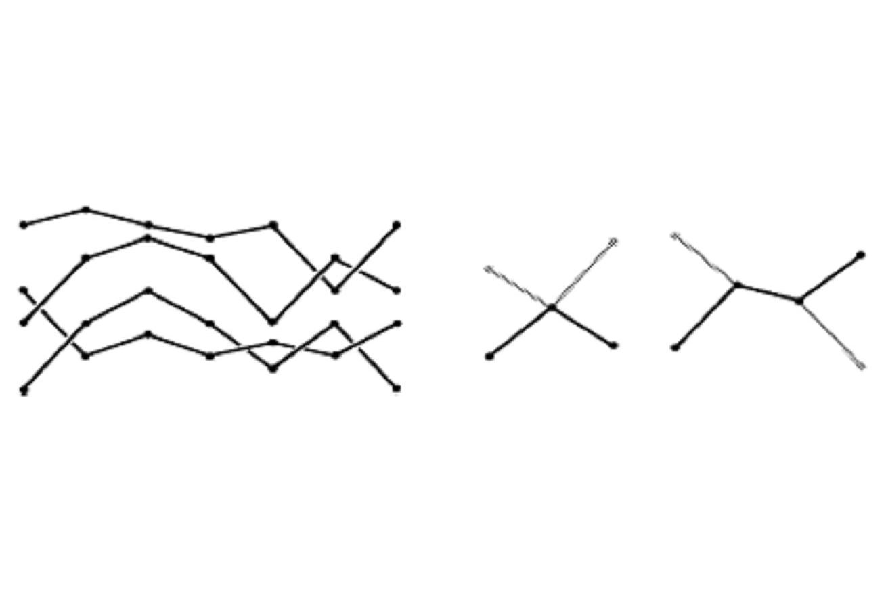
\epsfig{file=images/Fig2Kyoto2.pdf, scale=0.25}\caption{A discretized $\mathscr D_6^4$ (note: left and right
            hand sides are identified [left]; two types of singular discretized braids: a simple
            tangency and a high-order contact[right].}
        \end{figure}
\end{frame}
\begin{frame}{Discretized braid diagrams}
    \begin{block}{Definition}
        The space of {\em period $d$ discrete diagrams on $n$ strands\/}
        denoted by $\mathscr D_d^n$ is the space of all pairs $(\vu,
        \tau)$, \pause where $\tau$ is a permutation on $n$ elements \pause and
        $\vu=\{u^\alpha\}_{\alpha=1}^n$ is an unordered collection of
        vectors $u^\alpha=(u_i^\alpha)_{i=0}^d$,\pause i.e. {\em strands\/}
        such that:
        \begin{enumerate}
        \item Each strand consists of $d+1$ anchor points: $\vu^\alpha=(u_0^\alpha, \dots u_d^\alpha)\in
        \R^{d+1}$;\pause
        \item {\color{red}{(Periodicity)}\/}: $u_d^\alpha= u_0^{\tau(\alpha)}$;\pause
        \item {\color{red}{(Transversality)}\/}: for any $\alpha\neq \alpha'$ such
        that $u_i^\alpha=u_i^{\alpha'}$ for some $i$
        \[
        (u_{i-1}^\alpha - u_{i-1}^{\alpha'})(u_{i+1}^\alpha-
        u_{i+1}^{\alpha'})<0.
        \]
        \end{enumerate}
        \end{block}
\end{frame}
\begin{frame}
        \begin{block}{Notation}
            $[\vu]$ denotes the discrete braid class of a discrete braid
            diagram $\vu$.
        \end{block}
       \begin{figure}\label{fig:PLdiagram}
        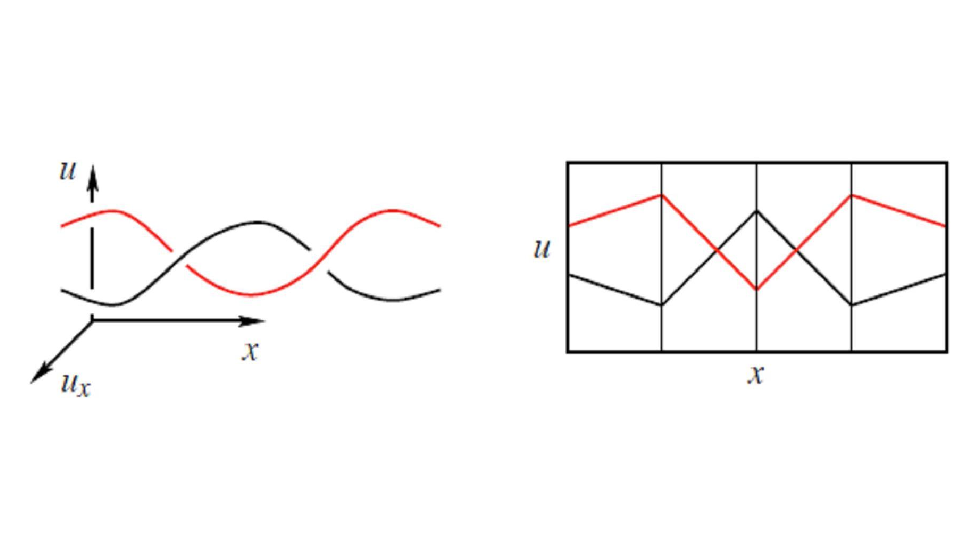
\epsfig{file=images/Fig19Wojcik2.pdf, scale=0.4}\caption{A braid on two strands [left]. The braid diagram
        (Piecewise linear representant of the class of the two dimensional projection of the
        braid) [right].}
        \end{figure}
\end{frame}
\begin{frame}
        \begin{figure}\label{fig:fig1Inve}
        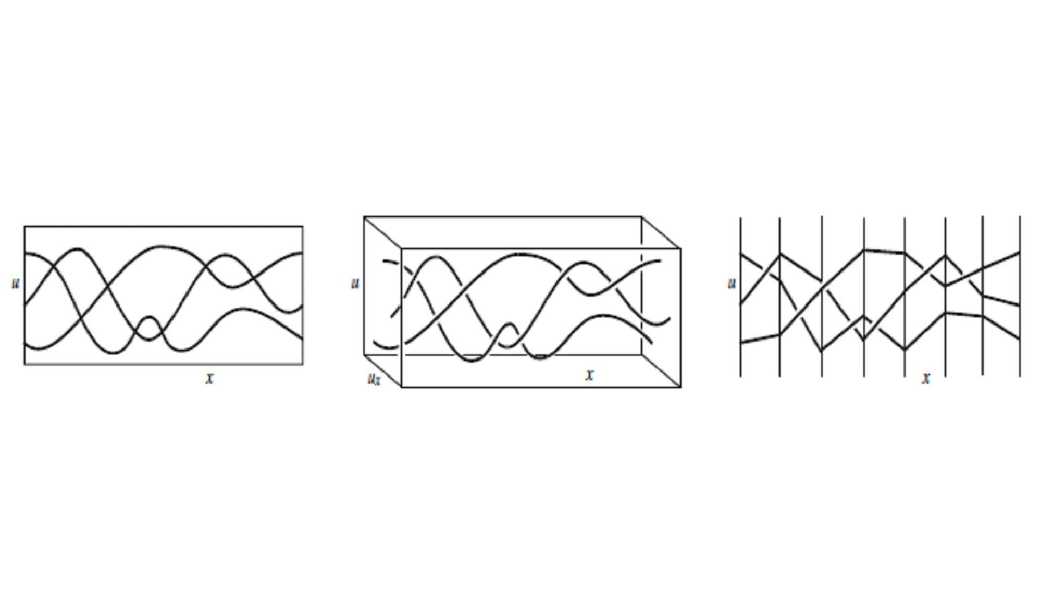
\epsfig{file=images/Fig1Inventiones2.pdf, scale=0.5}\caption{Curves on the (x,u)-plane [left] lift to a braid [center]
        which is then discretized [right]. In a discrete isotopy, one slides the anchor points vertically.}
        \end{figure}
\end{frame}
\begin{frame}{Discretization}
    \begin{block}{DISC and PL}
        If $\vu \in \Omega^n$ the period $d$ discretization is
        {\color{blue}{
        \[
        DISC_d(\vu):={u^\alpha(i/d)}_i^\alpha
        \]}\/}
        \pause
        Conversely, given a discrete braid $\vu\in \mathscr D_n^d$ we
        can associate a PL-braid diagram:\pause
        {\color{red}{
        \[
        PL(u^\alpha)(x):=u^\alpha_{\lfloor d\cdot x\rfloor}+ (d\cdot x-\lfloor d\cdot
        x\rfloor)(u^\alpha_{\lceil d\cdot x\rceil}-u^\alpha_{\lfloor d\cdot x\rfloor}).
        \]}\/}
    \end{block}
\end{frame}
\begin{frame}{Back and Forth}
    \begin{block}{...if $d$ is sufficiently large!}
        \begin{lem}
            Let $\vu \in \Omega^n$ and $\vv \in D_d^n$.
            \begin{itemize}
            \item PL sends the discrete braid class $[\vv]$ to a well
            defined topological braid class $\{PL(\vv)\}$.
            \item For $d$ sufficiently large, $\{PL(DISC_d(\vu))\}=\{\vu\}$.
            \end{itemize}
            \end{lem}
    \end{block}
\end{frame}
\subsection{Word length and linking number}
\begin{frame}{Admissibility and length}\pause
    \begin{block}{Braiding data are lost if the discretization is too coarse}
            A discretization period $d$ is {\color{blue}{admissible}\/} for
            $\vu \in \Omega^n$ if
            \[
            \{PL(DISC(\vu))\}=\{\vu\}.
            \]
        \end{block}\pause
        \begin{block}{The length}
            The {\color{blue}{length}\/} of a topological braid $\vu\in \Omega^n$, denoted by
            $\iota(\vu)$, \pause is defined to be the {\color{red}{total number of intersections
            in the braid diagram}.\/} \pause If $\vu \in \mathscr D_d^n$ is  a
            discrete braid, then $\iota(\vu):=\iota(PL(\vu))$.
    \end{block}
\end{frame}
\begin{frame}{Singular discretized braids}
    \begin{block}{Discriminant}\pause
    For {\color{blue}{topological braids}\/}, a {\color{red}{singular braid}\/} arises
    when any strands intersect. \pause For a {\color{blue}{discretized
    braid}\/}
    $\vu$, the {\color{red}{singular braids}\/} are defined to be those braids at
    which anchor points on two different strands coincide in a
    non-transverse fashion:\pause
    {\color{magenta}{
    \begin{eqnarray*}
        \Sigma :=\left\{\vu: \ u_i^\alpha=u_i^{\alpha'}\ \textrm{for some}\ i \ \textrm{and}\ \alpha \neq \alpha',\
        \textrm{and}\right.\\
        \left.  (u_{i-1}^\alpha - u_{i-1}^{\alpha'})(u_{i+1}^\alpha- u_{i+1}^{\alpha'})\geq
        0\right\}.
        \end{eqnarray*}}\/}
    \end{block}\pause
    The set $\Sigma$ carves $\mathscr D_d^n$ into components which
    are the discretized braid classes.
\end{frame}
\begin{frame}{Dynamics}
    \begin{block}{A parabolic relation}\pause
        of period $d$ is a sequence of maps $\mathscr R=\{\mathscr R_i:\R^3 \to
        \R\}$, $i=1, \dots, d$, such that $\partial_1 \mathscr R_i >0$ and
        $\partial_3 \mathscr R_i \geq 0$ for every $i$. \pause
        \end{block}
        \begin{block}{Applications}\pause
        This include discretization of uniform parabolic PDE's, as well
        as a variety of other systems.
        \end{block}
\end{frame}
\begin{frame}{Braid-theoretic comparison principle}
    \begin{block}{Parabolic flow}\pause
    Given a discretized braid $\vu=\{u_i^\alpha\}$ and a parabolic
    relation $\mathscr R$, one evolves braid according to the
    equation
    \[
    \dfrac{d}{dt}(u_i^\alpha)= \mathscr R_i(u_{i-1}^\alpha, u_i^\alpha,
    u_{i+1}^\alpha).
    \]
    \end{block}\pause
    \begin{block}{Stationary solutions}\pause
    corresponds to the braids $\vu$ such that $\mathscr R_i(\vu)=0$
    for all $i$. \pause

    {\color{blue}{The parabolic relation $\mathscr R$ induces a flow on $\mathscr D_d^n$ which
    respects a braid-theoretic comparison principle}.\/}
    \end{block}
\end{frame}
\begin{frame}{A crucial result}\pause
    \begin{block}{The algebraic length is a Lyapunov function}
        Let $\mathscr R$ be any parabolic relation and $\vu \in \Sigma$
        any singular braid. Then the flowline $\vu(t)$ of $\mathscr R$
        passing through $\vu=\vu(0)$ leaves  a neighborhood of $\Sigma$
        in forward and backward time so as to strictly decrease the
        algebraic length of $\vu(t)$ in the braid group as $t$ passes
        through zero.
    \end{block}
        \begin{figure}\label{fig:crossing}
        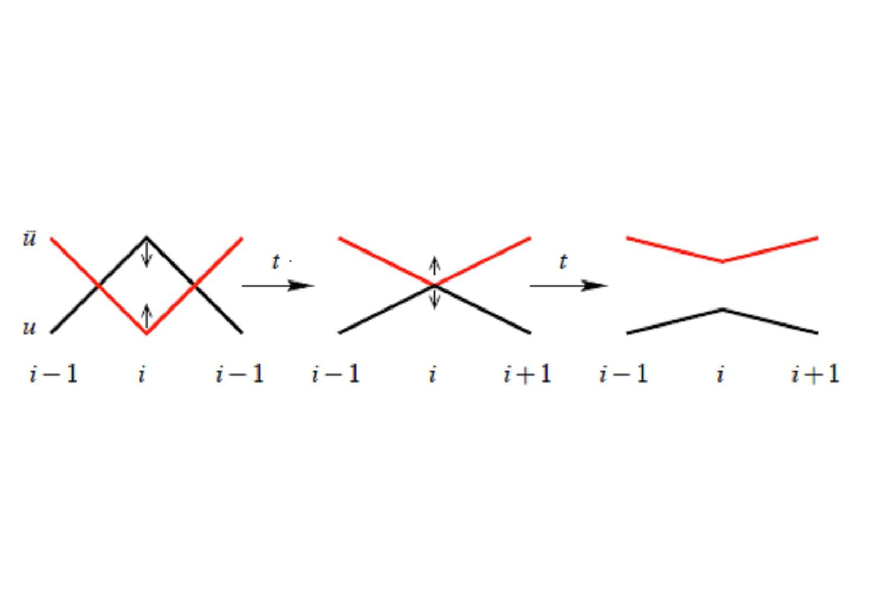
\epsfig{file=images/Fig112Wojcik2.pdf, scale=0.3}\caption{Along the evolution of the parabolic flow crossing can be
        destroyed, not created.}
        \end{figure}
\end{frame}
\begin{frame}{Proof}
    \begin{block}{an idea}
    \begin{figure}\label{fig:idea}
        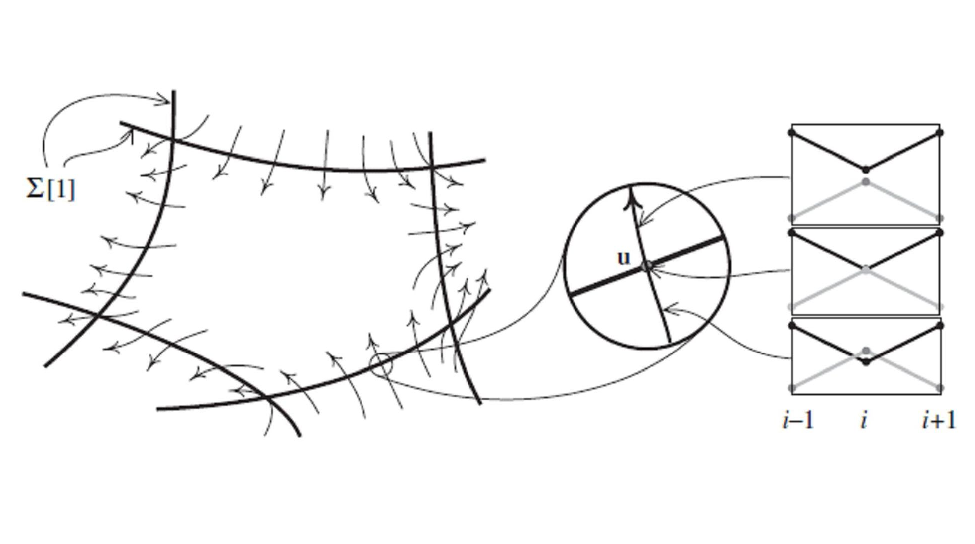
\epsfig{file=images/Fig2Inventiones2.pdf, scale=0.3}\caption{A schematic picture of a parabolic flow on
        a braid class. $\Sigma$ denotes the set of singular braids (boundary of the class). A parabolic flow on a discretized
        braid class is transverse to the boundary faces. The local linking of strands decreases strictly along the
        flowlines at a singular braid $\vu$.}
        \end{figure}
    \end{block}
\end{frame}
\subsection{Homotopic braid index as a Conley index}
\begin{frame}{The index}
    \begin{block}{Relative discretized braids}
        Given a period $d$ braid $\vv$, we denote by $\mathscr D_d^n
        rel\vv$ the space of all $n$ strands, period $d$ discretized braid
        which have $\vv$ has sub-braid.
        \end{block}\pause
    \begin{block}{Properness and boundedness}\pause
        The discretized relative braid class $[\vu rel \vv]$ is {\color{red}{proper}\/}
        if no free strands of $\vu$ can collapse onto $\vv$ or onto each
        other.\pause \\
        It is {\color{red}{bounded}\/} if there exists a uniform bound on all
        representatives $\vu$ of the equivalence class, i.e. if $\{\vu
        rel \vv\}$ is a bounded set in $\bar \Omega^n$.
    \end{block}
\end{frame}
\begin{frame}{Picture...}
\begin{figure}\label{fig:improper_Bounded}
        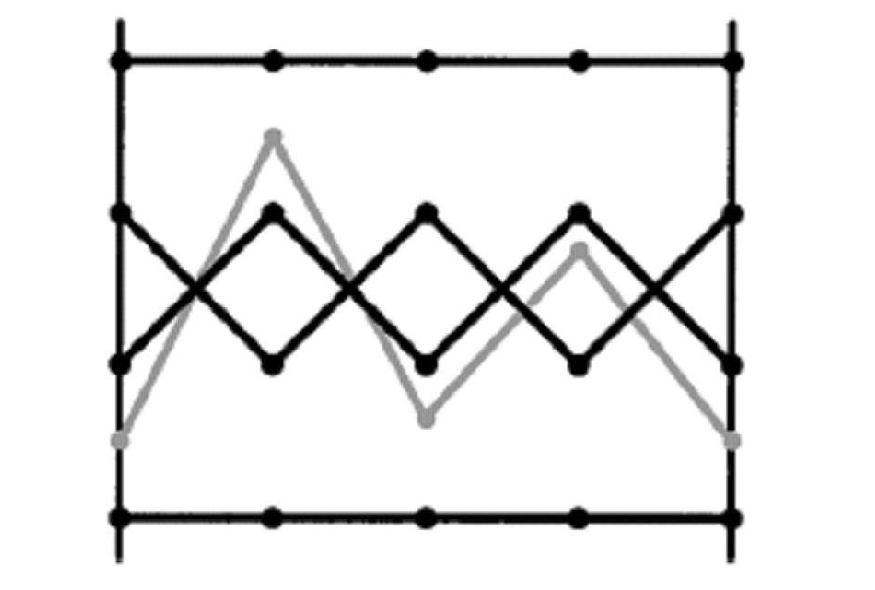
\epsfig{file=images/Fig4Inventiones22.pdf, scale=0.3}\caption{Improper and bounded relative braid class.}
        \end{figure}
\end{frame}
\begin{frame}{...One more picture}
\begin{figure}\label{fig:proper_Bounded}
        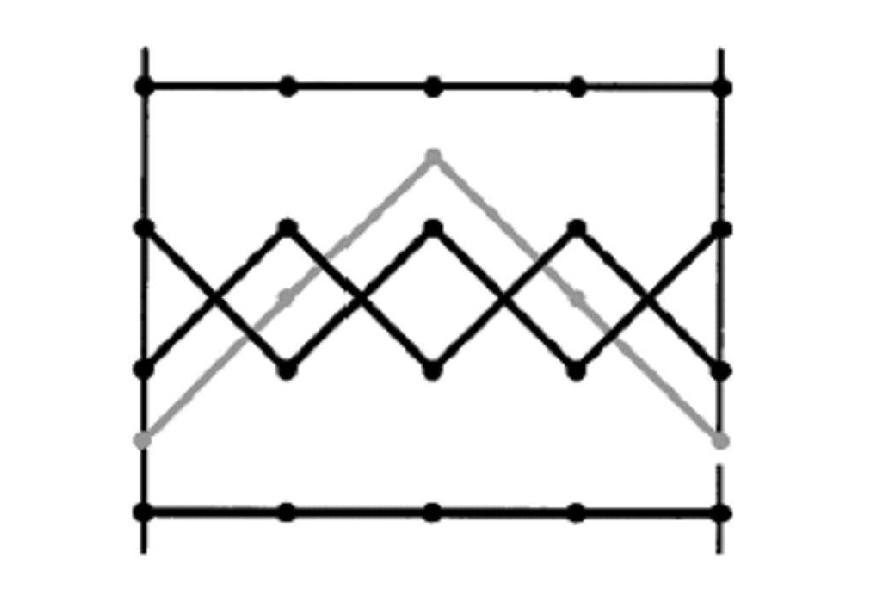
\epsfig{file=images/Fig4Inventiones21.pdf, scale=0.3}\caption{Proper and bounded relative braid class.}
        \end{figure}
\end{frame}
\begin{frame}{Homotopy braid index}
    \begin{block}{as Conley index of the braid class}\pause
        Choose any $\mathscr R$ which fixes $\vv$. Define $\mathscr E$
        to be those braids on the boundary of $[\vu rel \vv]$ along
        which the evolution under the flow of $\mathscr R$ exits the
        braid class.\pause

        The {\color{red}{homotopy braid index}\/} is defined to be the pointed homotopy
        class:\pause
        {\color{blue}{
        \[
        \vh([\vu rel\vv]):=([\vu rel \vv]/\mathscr E, \{\mathscr E\}).
        \]}\/}
    \end{block}
\end{frame}
\begin{frame}{Conley homology}
    \begin{oss}\pause
    Although the homotopy type of a quotient of a braid class seems
    difficult to compute, the homology $CH_*([\vu rel \vv])$ is both
    {\color{red}{efficacious}\/} and {\color{red}{computable}.\/}
    \end{oss}
\end{frame}
\begin{frame}{An example}
\begin{figure}\label{fig:example}
        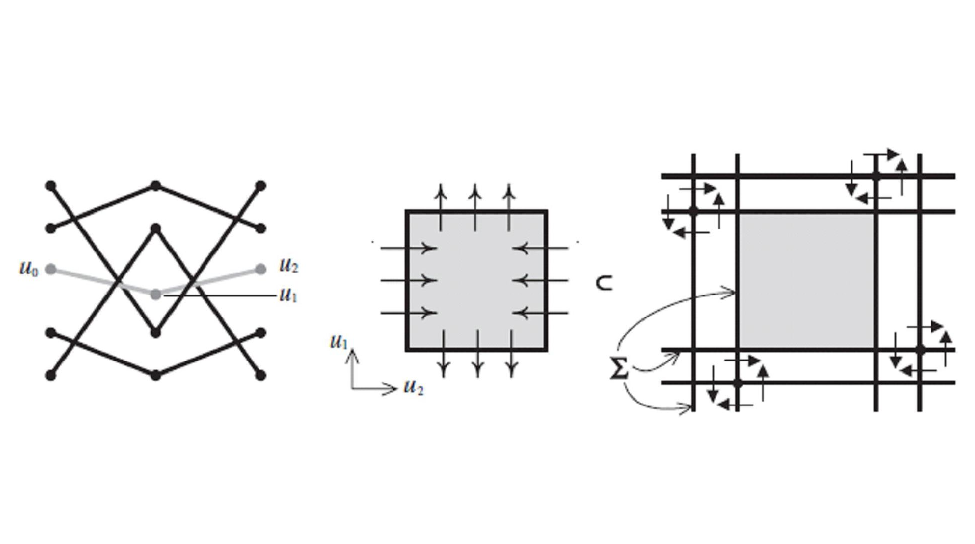
\epsfig{file=images/Fig5Inventiones2.pdf, scale=0.3}\caption{The braid in this Example [left]
        and the assocaited configuration space with parabolic flow [middle]. On the right is an expanded view
         of $\mathscr D_2^1 rel \vv$ where the fixed points of the flow correspond to the four fixed strands in the
         skeleton $\vv$. The braid class adjacent to these fixed points are not proper.}
        \end{figure}
\end{frame}

\subsection{A forcing theorem}
\begin{frame}{Topological content}
    \begin{thm}
        The homotopy braid index is a topological invariant of
        braids.
    \end{thm}
    \begin{thm}{\color{red}{(A forcing result)}}
    Let $\mathscr R$ be a parabolic relation such that:
    \begin{enumerate}
    \item[(i)] {\color{blue}{gradient-type}\/};
    \item[(ii)] {\color{blue}{dissipative}\/} (roughly, that large solutions are {\em
    repelled \/} from infinity). If $\mathscr R$ fixes a
    discretized braid $\vv$ which is not in the trivial braid class
    (that is, if it has any crossings whatsoever), then there are an
    infinite number of distinct braid classes for multiple periods
    which arise as stationary solutions of $\mathscr R$.
    \end{enumerate}
    \end{thm}
\end{frame}
\begin{frame}{Applications}
    \begin{block}{Second order Lagrangians}
        Consider a {\em second order Lagrangian\/} $L=L(u, u_x,
        u_{xx})$, such as found in Swift-Hohenberg equations:
        \[
        L= \dfrac12(u_{xx})^2- (u_x)^2 + \dfrac{1-\alpha}{2}u^2 +
        \dfrac{u^4}{4}.
        \]
    \end{block}\pause
    \begin{block}{How to find periodic orbits?}\pause
        In the case of second order Lagrangian, the problem translates
        to finding periodic orbits of a Hamiltonian flow on energy-level
        three manifold.
    \end{block}
\end{frame}
\begin{frame}{When the compactness is lost!}
    \begin{block}{Symplectic references}
        This problem is extremely delicate, requiring refined techniques
        as pseudoholomorphic curves (as developed by Gromov and Hofer)
        and the contact homology of Eliashberg, Givental, Hofer,
        Wysocky, Zehnder etc.
    \end{block} \pause
    \begin{oss}
        All of these techniques strongly
        depends on some compactness (Palais-Smale) of the energy level and upon a
        topological convexity (an invariant contact structure).\pause Neither
        of these conditions are guaranteed for a general second-order
        Lagrangian: indeed the compactness is always lost.
    \end{oss}
\end{frame}
    %By restricting to systems which satisfy a {\color{red}{twist
%    condition}\/} (a mild variational hypothesis), it is possible to
\begin{frame}{The main result}
    \begin{thm}
    Let $L$ be as above. Then, at any regular energy level, the
    existence of a single periodic orbit which traces out a non
    trivial curve in the $(u, u_x)$-plane implies the existence of
    {\color{red}{infinitely}\/} many others at this energy level.
    \end{thm}
\end{frame}

%%%%%%%%%%%%%%%%%%%%%%%%%%%%%%%%%%%%%%%%%%%%%%%%%%%%%%%%%%%%%%%%%%%%%%%%%%%%%%%%%%%%%%%%%%%%%%%%%%%%%%%%%%%%%%%%%%%
\appendix
\section{}
\begin{frame}{}
\begin{center}
\begin{Large}
\alert{Thank you for your attention!}
\end{Large}
\end{center}
\end{frame}
\end{document}
